\documentclass[10pt,conference,compsocconf]{IEEEtran}

\usepackage{hyperref}
\usepackage{graphicx}	% For figure environment


\begin{document}
\title{Machine Learning Course CS-433 - Project 1 report}

\author{
  Luca Bataillard, Julian Blackwell, Changling Li\\
  \textit{School of Computer and Communication Sciences, EPFL}
}

\maketitle

\section{Introduction}
The aim of this project is to learn to use the concepts of machine learning presented in the lectures and practiced in the labs on a
real-world dataset. In the following sections, we will present every step taken such as exploratory data analysis to understand the dataset, before applying feature processing to clean the dataset and extract more meaningful information. We implemented the machine learning methods from the set of regression analysis such as linear regression, ridge regression and logistic regression using gradient descent, stochastic gradient descent or normal equations. Then, we analyzed the results produced by these different methods and continuously improved the models, by finally choosing the best one. This project was done in the context of a recent popular machine learning challenge - finding the Higgs boson -, using original data from CERN~\cite{higgs}.

\section{Exploratory data analysis}
\label{sec:structure-paper}

In order to learn about our dataset, We first read appendix B of the original Higgs paper~\cite{higgs} and discovered several key points : 

\begin{itemize}

\item The event label (string) $y_i \in \{s, b\}$ (s for signal, b for background)
\item The variables prefixed with PRI (for PRImitives) are “raw” quantities about the bunch collision as measured by the detector.
\item The variables prefixed with DER (for DERived) are quantities computed from the primitive features
\item Undefined values are denoted by \texttt{-999.0}, which is outside the normal range of all variables.
\item All variables are floating point and continuous, apart from 
\texttt{PRI\_jet\_num}, which ranges in $\{0, 1, 2, 3\}$

\end{itemize}
\ \\
Then, we did some basic data checks such as making sure the labels correspond either to 1 (which corresponds to s) and to -1 (for b). Then, we inspected the size of the dataset which contains 250'000 data samples with 30 feature columns. With a dataset of this type (n $>>$ p), we will not face the challenges of a high-dimensional data. Then, we analyzed our data in the following subsections.
\ \\

\subsection{Inspecting the features} 
We inspected the first values of the features to confirm the previous claims. As expected, we noticed some \texttt{-999.0} values and \texttt{PRI\_jet\_num} is indeed discrete the only feature that has discrete values. All the other variables are floating point and continuous.
\subsection{Summary statistics} 
By computing the summary statistics on the data, we noticed that undefined values are not present in all columns. However, in columns where they are present, they comprise a large proportion of the data.
We also noticed that each feature follows a very different distribution. 
\subsection{Correlation between features} 
To check if there are obvious relationships or correlation between the features, we implemented the function \texttt{plot\_corr\_matrix} from \texttt{implementations.py} in order to have a visual representation of the lower triangle of the Pearson correlation matrix between the features. The triangle contains all the Pearson correlation coefficients which give a measure of linear correlation between the features. We noticed some features are strongly correlated to each other (see Fig. \ref{corr_matrix}). 


\section{Feature processing}
In order to get the most out of our data and to ease model computational cost for the best possible results from our models, we applied some feature processings.

\subsection{Handle undefined values}
As mentioned in the exploratory data analysis, we noticed a few features that have over $70\%$ invalid values. We therefore decided to remove these columns to allow for more robust models, with the help of the function \texttt{handle\_invalid}. The removed features were :\texttt{DER\_deltaeta\_jet\_jet, DER\_mass\_jet\_jet, DER\_prodeta\_jet\_jet, DER\_lep\_eta\_centrality, PRI\_jet\_subleading\_pt, PRI\_jet\_subleading\_eta, PRI\_jet\_subleading\_phi}.

Moreover, we also handled the other undefined values by replacing them with the mean of their respective columns, again with the help of the function \texttt{handle\_invalid}.

\subsection{Remove correlated features}
From Fig. \ref{corr_matrix}, we observed some features that are strongly correlated with others. These features contribute very less in predicting the output but increase the computational cost. We therefore made the decision to discard the features that are characterized by a correlation coefficient higher than 0.8. The ones that are concerned by this criteria are the features : \texttt{DER\_pt\_h, DER\_sum\_pt, PRI\_met\_sumet}.

\subsection{Standardization}
We noticed in the summary statistics that there are some features that are measured at different scales; they have large differences between their ranges or simply they are measure in different measurement units. This means that each feature could not contribute equally to the model fitting and might end up creating a bias. We have thus chosen to standardize or Z-score normalize our data by subtracting the mean and dividing by the standard deviation for each value of each feature with the help of the function \texttt{standardize} : $standardized\_feature = \frac{feature - mean(feature)}{standard\_deviation(feature)}$





\begin{enumerate}
\item State the problem.
\item Say why it is an interesting problem.
\item Say what your solution achieves.
\item Say what follows from your solution.
\end{enumerate}

please \emph{use a
  spell checker}.


Use examples and illustrations to clarify ideas and results. For
example, by comparing Figure~\ref{fig:denoise-fourier} and
Figure~\ref{fig:denoise-wavelet}, we can see the two different
situations where Fourier and wavelet basis perform well. 

\subsection{Models and Methods}
The models and methods
section should describe what was
done to answer the research question, describe how it was done,
justify the experimental design, and
explain how the results were analyzed.

The model refers to the underlying mathematical model or structure which 
you use to describe your problem, or that your solution is based on. 
The methods on the other hand, are the algorithms used to solve the problem. 
In some cases, the suggested method directly solves the problem, without having it 
stated in terms of an underlying model. Generally though it is a better practice to have 
the model figured out and stated clearly, rather than presenting a method without specifying 
the model. In this case, the method can be more easily evaluated in the task of fitting 
the given data to the underlying model.

The methods part of this section, is not a step-by-step, directive,
protocol as you might see in your lab manual, but detailed enough such
that an interested reader can reproduce your
work.

The methods section of a research paper provides the information by
which a study's validity is judged.
Therefore, it requires a clear and precise description of how an
experiment was done, and the rationale
for why specific experimental procedures were chosen.
It is usually helpful to
structure the methods section by:
\begin{enumerate}
\item Layout the model you used to describe the problem or the solution.
\item Describing the algorithms used in the study, briefly including
  details such as hyperparameter values (e.g. thresholds), and
  preprocessing steps (e.g. normalizing the data to have mean value of
  zero).
\item Explaining how the materials were prepared, for example the
  images used and their resolution.
\item Describing the research protocol, for example which examples
  were used for estimating the parameters (training) and which were
  used for computing performance.
\item Explaining how measurements were made and what
  calculations were performed. Do not reproduce the full source code in
  the paper, but explain the key steps.
\end{enumerate}

\subsection{Results}

Organize the results section based on the sequence of table and
figures you include. Prepare the tables and figures as soon as all
the data are analyzed and arrange them in the sequence that best
presents your findings in a logical way. A good strategy is to note,
on a draft of each table or figure, the one or two key results you
want to address in the text portion of the results.
The information from the figures is
summarized in Table~\ref{tab:fourier-wavelet}.

\begin{table*}[htbp]
  \centering
  \begin{tabular}[c]{|l||l|l|l|}
    \hline
    Basis&Support&Suitable signals&Unsuitable signals\\
    \hline
    Fourier&global&sine like&localized\\
    wavelet&local&localized&sine like\\
    \hline
  \end{tabular}
  \caption{Characteristics of Fourier and wavelet basis.}
  \label{tab:fourier-wavelet}
\end{table*}

When reporting computational or measurement results, always
report the mean (average value) along with a measure of variability
(standard deviation(s) or standard error of the mean).


\section{Tips for Good Software}
\label{sec:tips-software}

There is a lot of literature (for example and
) on how to write software. It is not the
intention of this section to replace software engineering
courses. However, in the interests of reproducible
research, there are a few guidelines to make your
reader happy:
\begin{itemize}
\item Have a \texttt{README} file that (at least) describes what your
  software does, and which commands to run to obtain results. Also
  mention anything special that needs to be set up, such as
  toolboxes\footnote{For those who are
  particularly interested, other common structures can be found at
  \url{http://en.wikipedia.org/wiki/README} and
  \url{http://www.gnu.org/software/womb/gnits/}.}.
\item A list of authors and contributors can be included in a file
  called \texttt{AUTHORS}, acknowledging any help that you may have
  obtained. For small projects, this information is often also
  included in the \texttt{README}.
\item Use meaningful filenames, and not \texttt{temp1.py},
  \texttt{temp2.py}. 
\item Document your code. Each file should at least have a short
  description about its reason for existence. Non obvious steps in the
  code should be commented. Functions arguments and return values should be described.
\item Describe how the results presented in your paper can be reproduced.
\end{itemize}


\subsection{\LaTeX{} Primer}
\label{sec:latex-primer}

\LaTeX{} is one of the most commonly used document preparation systems
for scientific journals and conferences. It is based on the idea
that authors should be able to focus on the content of what they are
writing without being distracted by its visual presentation.
The source of this file can be used as a starting point for how to use
the different commands in \LaTeX{}. We are using an IEEE style for
this course.

\subsubsection{Installation}

There are various different packages available for processing \LaTeX{}
documents.
On OSX use Mac\TeX{}
(\url{http://www.tug.org/mactex/}). On Windows, use for example Mik\TeX{} (\url{http://miktex.org/}).

\subsubsection{Compiling \LaTeX{}}
Your directory should contain at least~4 files, in addition to image
files. Images should be in \texttt{.png}, \texttt{.jpg} or
\texttt{.pdf} format.
\begin{itemize}
\item IEEEtran.cls
\item IEEEtran.bst
\item groupXX-submission.tex
\item groupXX-literature.bib
\end{itemize}
Note that you should replace groupXX with your chosen group name.
Then, from the command line, type:
\begin{verbatim}
$ pdflatex groupXX-submission
$ bibtex groupXX-literature
$ pdflatex groupXX-submission
$ pdflatex groupXX-submission
\end{verbatim}
This should give you a PDF document \texttt{groupXX-submission.pdf}.

\subsubsection{Equations}

There are three types of equations available: inline equations, for
example $y=mx + c$, which appear in the text, unnumbered equations
$$y=mx + c,$$
which are presented on a line on its own, and numbered equations
\begin{equation}
  \label{eq:linear}
  y = mx + c
\end{equation}
which you can refer to at a later point (Equation~(\ref{eq:linear})).

\subsubsection{Tables and Figures}

Tables and figures are ``floating'' objects, which means that the text
can flow around it.
Note
that \texttt{figure*} and \texttt{table*} cause the corresponding
figure or table to span both columns.



\section{Summary}

The aim of a scientific paper is to convey the idea or discovery of
the researcher to the minds of the readers. The associated software
package provides the relevant details, which are often only briefly
explained in the paper, such that the research can be reproduced.
To write good papers, identify your key idea, make your contributions
explicit, and use examples and illustrations to describe the problems
and solutions.

\section*{Acknowledgements}
The author thanks Christian Sigg for his careful reading and helpful
suggestions.

\bibliographystyle{IEEEtran}
\bibliography{literature}


\begin{figure}[h]
  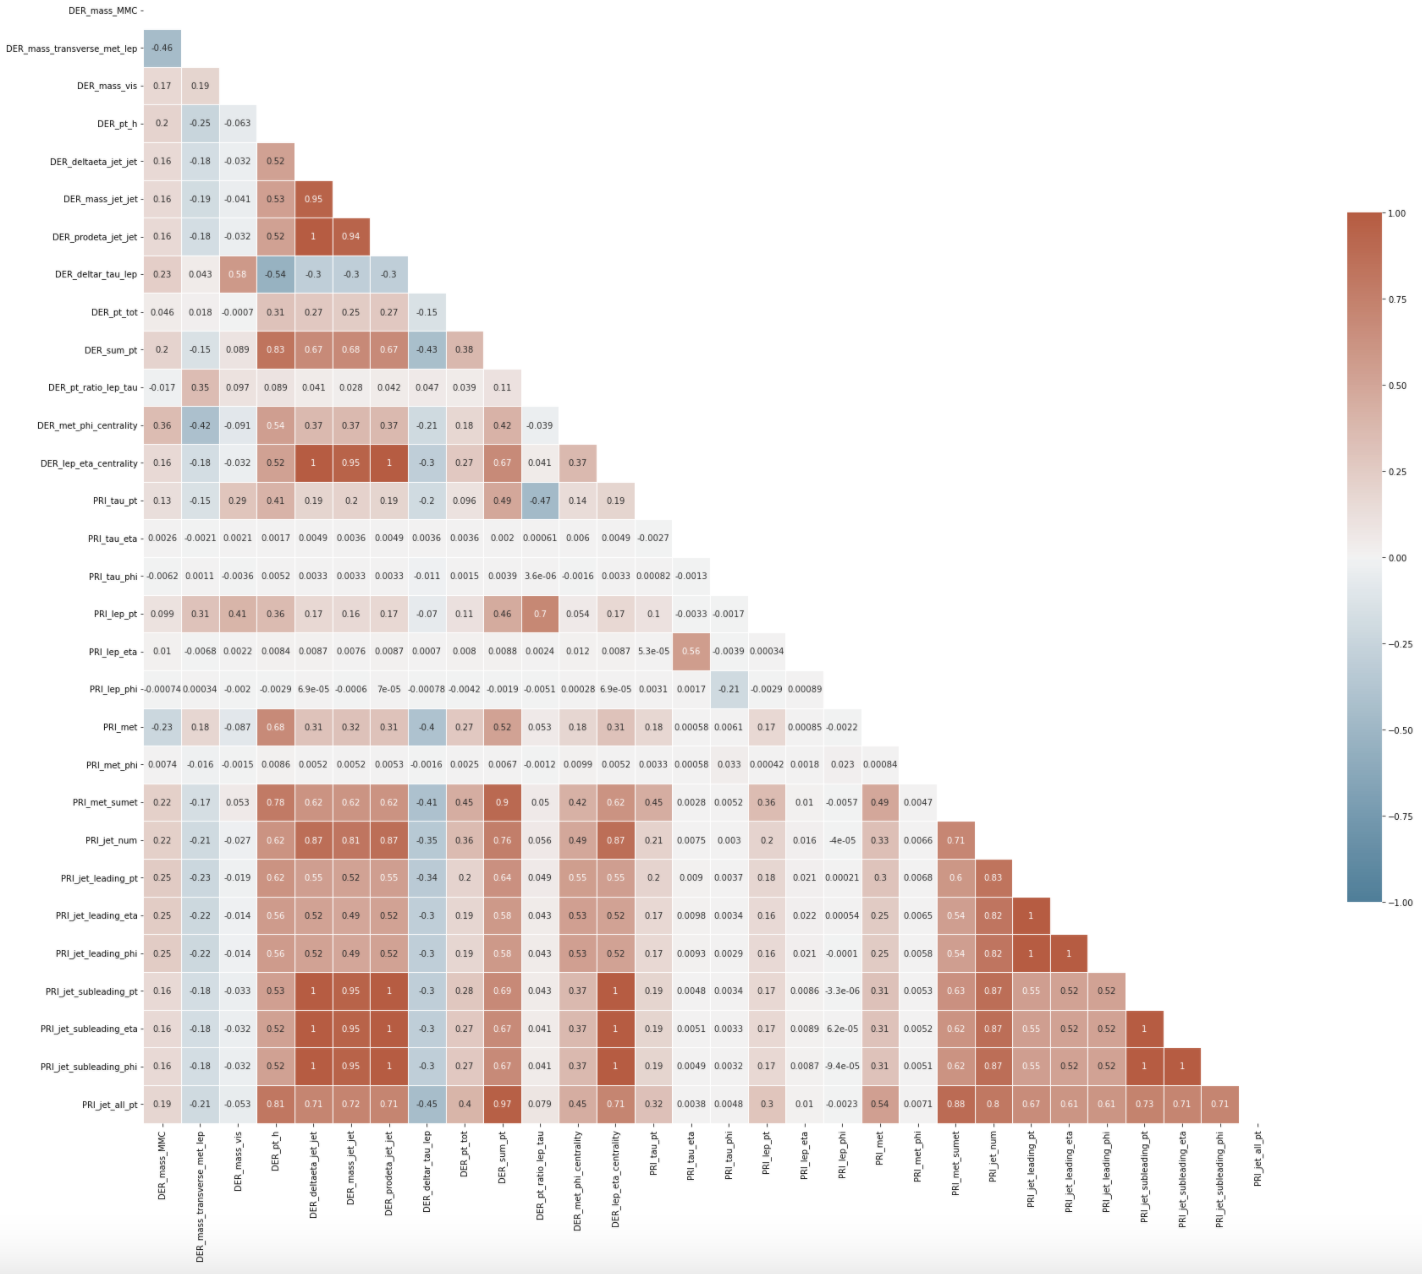
\includegraphics[scale = 0.75]{corr_matrix.png}
  \caption{Lower triangle of the Pearson correlation matrix between features}
  \label{corr_matrix}
\end{figure}

\end{document}
